% !TeX root = ../thuthesis-example.tex

\chapter{PROTOTYPE OF VR-IoT Research Platform}

\section{Platform requirements}
Firstly, we define the requirements our platform should follow:
\begin{enumerate}
\item Scalability. The performance of the platform should stay acceptable when the number of devices in our system increase;
\item Ease of use and testing. Since using Virtual Reality and IoT devices requires interacting with different kinds of elements, we need to provide a natural way of interacting with such objects. As for real-world devices we only need to implement sensor data collection, creating an API for virtual reality digital representation of such devices can be a challenge. Another important task is simulation of VR interactions on a computer for ease of testing;
\item Fault Tolerance. As if we are not developing the IoT devices themselves, platform should effectively handle faults coming from both sides (real and virtual worlds);
\item Simultaneous work. As in the real world, when several people can interact with an IoT system, each of the running instances of the platform should be able to run simultaneously and operate with the same data.
\end{enumerate}
The architecture of the platform has to be based on three layers, which we further modify and extend with extra connections: 
\begin{enumerate}
    \item Real-world IoT devices HUB. In order to collect the data from real-world devices, we need a special device responsible for receiving and sending the data to them. In commercial market, usually mobile phone apps have interface to interact with IoT devices (Mi Home APP, HomeKit App etc), but since we require using the data in virtual reality (which is a different interface), we need to operate with IoT sensors data on a special HUB, which can provide the data in a unified format (abstraction of sensors)
    \item Integration layer. This is the main part of the platform. Analyzing data coming from VR and from real world, integrating real-world devices data into VR and vice-versa, performing persistence and providing API for using the platform in research projects;
    \item Visualization layer. Interaction with digital IoT devices can be performed using VR headsets, AR devices or by simulating the touch, sight, gestures and other interactions. Our aim is to provide an API for developers to integrate their interaction techniques into this layer, but developing these techniques is not the focus of this research. 
\end{enumerate}

\section{Real-world IoT devices HUB}
To support different IoT devices in out platform, either a standalone or third-party software can be used. By analyzing the market, we have agreed on using a third-party software openHAB with a future upgrade to our own solution. The Hub we use runs on a server and is responsible for collecting and storing the data coming from IoT devices. Managing the data is performed through a web interface, while API is based on REST calls.

\section{Integration layer}
By receiving and sending unified data objects representing IoT devices sensor data using REST API calls, each of the running instances of the NUIX-Studio App (our platform) running in the Integration layer will operate with the same data, enabling simultaneous work.
Next step is to represent IoT devices data in virtual reality and perform computations for research. Since the platform should run smoothly on VR headsets and provide good UX, the computations should be performed on a high-performance PC, while interaction with virtual IoT devices is done by using VR headsets. 

\section{Visualization layer}
Since the platform purpose is to provide an API for research on IoT devices in VR, we decided to use Unity for interaction with virtual reality devices. First of all, by choosing Unity, we save time from developing our own 3D engine. Secondly, we can build the project for most of platforms and provide support for VR headsets. And thirdly, developers are already familiar with Unity development, and can integrate their research projects into the platform faster than if we used our own 3D engine.

\begin{figure}
  \centering
  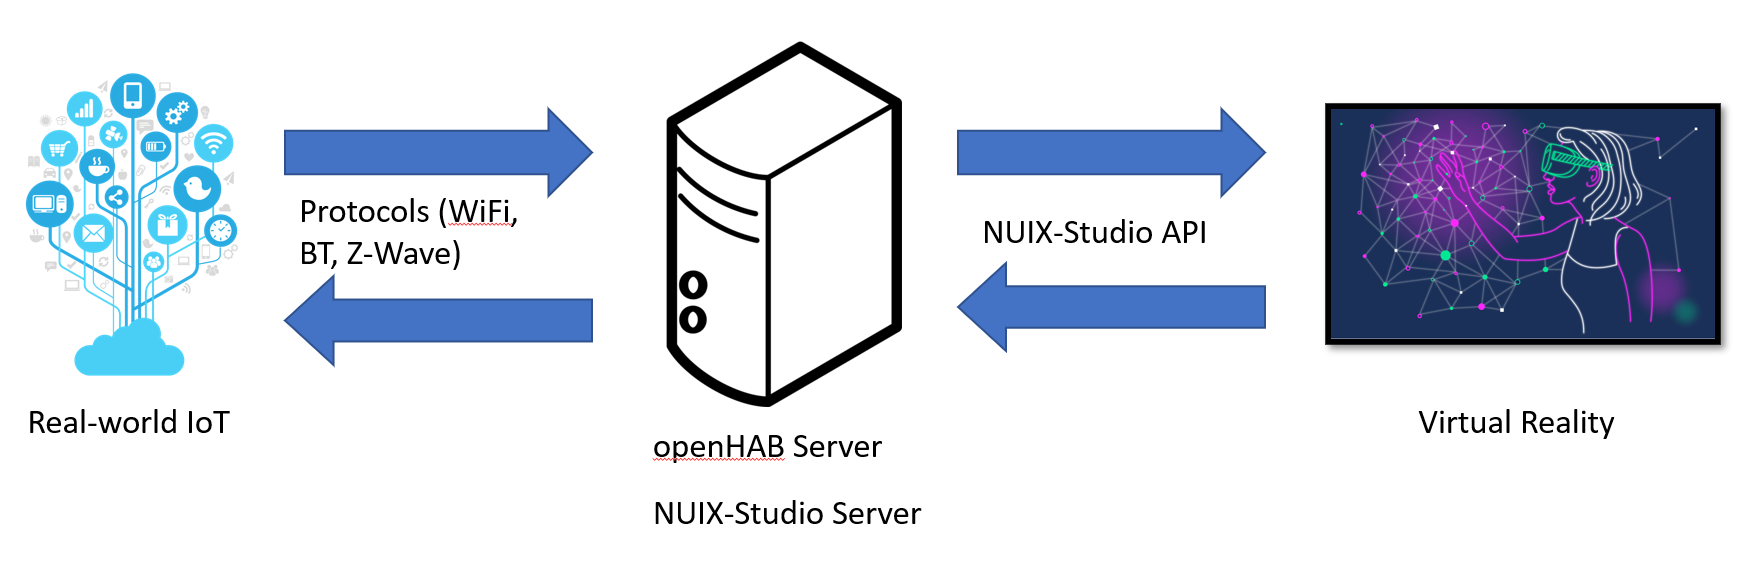
\includegraphics[width=0.6\linewidth]{figures/BasicPlatformStructure.png}
  \caption{Simplified structure of NUIX Studio. Real-world IoT devices HUB is openHAB server, while NUIX-Studio server is the main instance of NUIX-Studio APP responsible for the computations.}
  \label{fig:BasicPlatformStructure-figure}
\end{figure}

\section{Server Architecture}
\subsection{OpenHAB Server Structure}

Before we explain the structure of our server, we first give definitions for the base elements of openHAB:

Things are entities that can be physically added to a system. Things may provide more than one function (for example, a Z-Wave multi-sensor may provide a motion detector and also measure room temperature). Things do not have to be physical devices; they can also represent a web service or any other manageable source of information and functionality.

Things expose their capabilities through Channels. Whether an installation takes advantage of a particular capability reflected by a Channel depends on whether it has been configured to do so. When you configure your system, you do not necessarily have to use every capability offered by a Thing. You can find out what Channels are available for a Thing by looking at the documentation of the Thing's Binding.

Bindings can be thought of as software adapters, making Things available to your home automation system. They are add-ons that provide a way to link Items to physical devices. They also abstract away the specific communications requirements of that device so that it may be treated more generically by the framework.

Items represent capabilities that can be used by applications, either in user interfaces or in automation logic. Items have a State and they may receive commands.

The glue between Things and Items are Links. A Link is an association between exactly one Channel and one Item. If a Channel is linked to an Item, it is "enabled", which means that the capability the Item represents is accessible through that Channel. Channels may be linked to multiple Items and Items may be linked to multiple Channels.

\begin{figure}
  \centering
  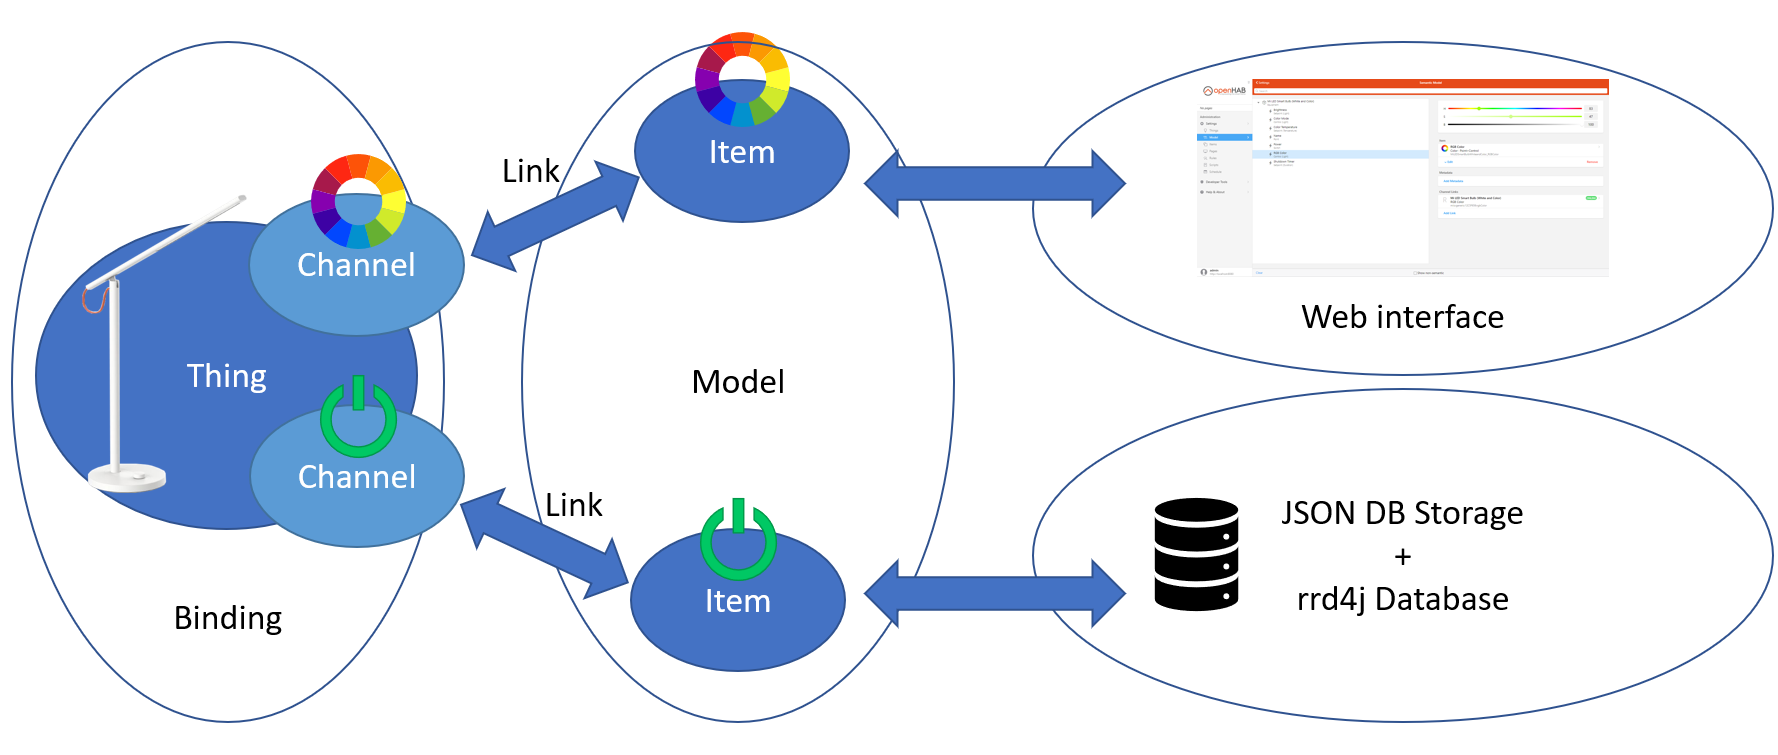
\includegraphics[width=0.9\linewidth]{figures/openHABServerStructure.png}
  \caption{Simplified structure of NUIX Studio. Real-world IoT devices HUB is openHAB server, while NUIX-Studio server is the main instance of NUIX-Studio APP responsible for the computations.}
  \label{fig:openHABServerStructure-figure}
\end{figure}

\begin{figure}
  \centering
  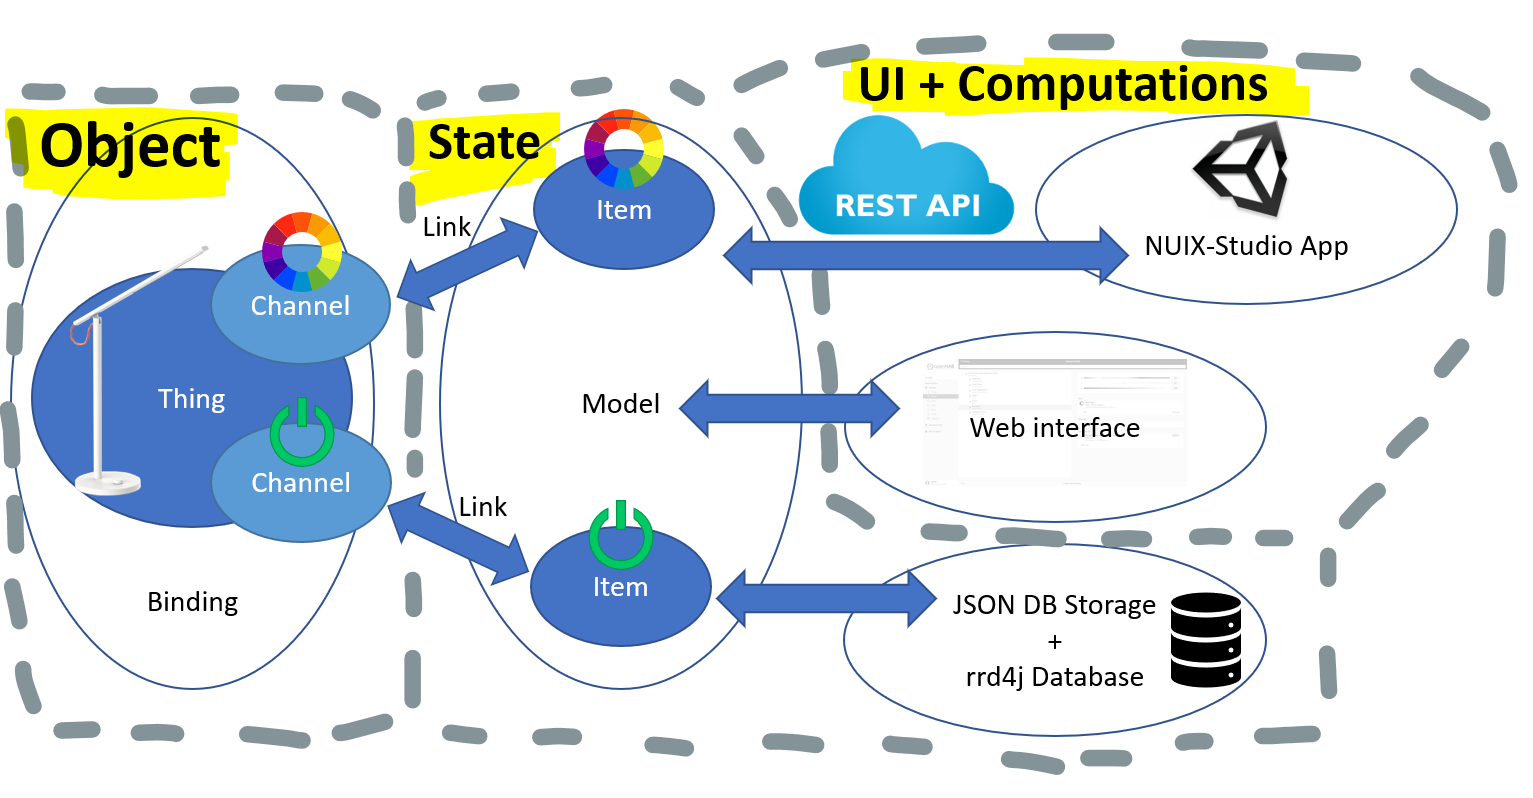
\includegraphics[width=0.9\linewidth]{figures/ExtendedServerStructure.png}
  \caption{Simplified structure of NUIX Studio. Real-world IoT devices HUB is openHAB server, while NUIX-Studio server is the main instance of NUIX-Studio APP responsible for the computations.}
  \label{fig:ExtendedServerStructure-figure}
\end{figure}

\section{Symbols}

As required by the national formatting standards, the template uses \pkg{unicode-math} for formatting mathematical symbols, which differs to the default used by LATEX. 

\begin{enumerate}
  \item Capital Greek letters are italic by default e.g. \cs{Delta}:$\Delta$。
  \item Increment symbol: $\increment$(U+2206)
  \item Vectors, matrices, tensors should be ITALIC, and BOLD using the \cs{symbf} command; for example: $\symbf{A}$, $\symbf{\alpha}$.
  \item For constants and special functions, use the \cs{symup} command. For example:
    $\symup{\pi} = 3.14\dots$; $\symup{e} = 2.718\dots$,
  \item Example of integrals and differentials: $\int f(x) \dif x$。
\end{enumerate}

For more usage of symbols, you could use the following references
\href{http://mirrors.ctan.org/macros/latex/contrib/unicode-math/unicode-math.pdf}{\pkg{unicode-math}}
\href{http://mirrors.ctan.org/macros/latex/contrib/unicode-math/unimath-symbols.pdf}{\pkg{unimath-symbols}}.

For units and metrics, it is recommended to use the following package:
\href{http://mirrors.ctan.org/macros/latex/contrib/siunitx/siunitx.pdf}{\pkg{siunitx}}
It can conveniently handle the space between Greek letters/numbers and the unit. For example:
\SI{6.4e6}{m},
\SI{9}{\micro\meter},
\si{kg.m.s^{-1}},
\SIrange{10}{20}{\degreeCelsius}。



\section{Mathematical formula}

You can use the following environments \env{equation} 和 \env{equation*} for mathematical formulae.

Please pay attention that round brackets should be included before and after referencing an equation: e.g. Equation \eqref{eq:example}.

\begin{equation}
  \frac{1}{2 \symup{\pi} \symup{i}} \int_\gamma f = \sum_{k=1}^m n(\gamma; a_k) \mathscr{R}(f; a_k)
  \label{eq:example}
\end{equation}

When there are multiple equations, please try to align them at the "equal" sign if possible. We recommend using the \env{align} environment.
For example:
\begin{align}
  a & = b + c + d + e \\
    & = f + g
\end{align}


\section{Mathematical axioms and proofs}

You can use \pkg{amsthm} or \pkg{ntheorem} packages to set up your axiom. After loading one of those package, the template will automatically setup the environments: \env{theorem} and \env{proof}

An example:
\begin{theorem}[Lindeberg--Lévy Central Limit Theorem]
  Set random variables $X_1, X_2, \dots, X_n$ i.i.d., with expectation mean of $\mu$ and variance $\sigma^2 \ne 0$. By formula, $\bar{X}_n = \frac{1}{n} \sum_{i+1}^n X_i$, we have
  \begin{equation}
    \lim_{n \to \infty} P \left(\frac{\sqrt{n} \left( \bar{X}_n - \mu \right)}{\sigma} \le z \right) = \Phi(z),
  \end{equation}
  where $\Phi(z)$ is the function of a normal distribution.
\end{theorem}
\begin{proof}
  Trivial.
\end{proof}

The template also provides the following environments: \env{assumption}、\env{definition}、\env{proposition}、
\env{lemma}、\env{theorem}、\env{axiom}、\env{corollary}、\env{exercise}、
\env{example}、\env{remar}、\env{problem}、\env{conjecture} 